\subsection{Disclaimer}\label{disclaimer}

I do not have any affiliation with any of the presented tools!

\begin{center}\rule{0.5\linewidth}{\linethickness}\end{center}

\subsection{Overview}\label{overview}

\begin{enumerate}
\def\labelenumi{\arabic{enumi}.}
\item
  Required Tools
\item
  \ldots{}
\end{enumerate}

--- .segue .dark

\subsection{Required Tools}\label{required-tools}

\begin{center}\rule{0.5\linewidth}{\linethickness}\end{center}

\subsection{Required Tools}\label{required-tools-1}

We make use of the following Tools/ R-packages

\begin{enumerate}
\def\labelenumi{\arabic{enumi}.}
\item
  RStudio
\item
  GitHub
\item
  Slidify (including Markdown)
\item
  googleVis
\end{enumerate}

\begin{center}\rule{0.5\linewidth}{\linethickness}\end{center}

\subsection{RStudio}\label{rstudio}

\begin{itemize}
\item
  Supposedly all of you have heard about RStudio.
\item
  First version (v0.92) of RStudio was published in February 2011.
\item
  Back then there were plenty of competing R editors, but these days
  RStudio became the quasi standard.
\item
  The popularity of RStudio is due to its large amount of included
  features.
\item
  RStudio is available as desktop and server version.
\item
  RStudio also powers `Shiny', a web application framework for R.
\item
  One not so common, but very useful feature is the project feature.
\end{itemize}

\begin{center}\rule{0.5\linewidth}{\linethickness}\end{center}

\subsection{GitHub}\label{github}

\begin{itemize}
\item
  Supposedly most of you also have heard about GitHub (or at least git)
\item
  git is a revision control system, initially developed 2005 by Linus
  Torvalds for the Linux kernel.
\item
  GitHub is a filehosting service (founded 2008) that is based on the
  git technology.
\item
  GitHub is designed especially for the development of larger software
  projects (branch, merge, fork).
\item
  It is getting more and more popular to keep R-packages only on GitHub
  and not to submit to Cran.
\item
  Researchers can apply for free private repositories via {[}GitHub
  education{]} (https://education.github.com/).
\item
  GitHub provides webspace for webpages via
  \hyperref[github-pages]{GitHub pages} (https://pages.github.com/).
\end{itemize}

\begin{center}\rule{0.5\linewidth}{\linethickness}\end{center}

\hyperdef{}{github-pages}{\subsection{GitHub pages}\label{github-pages}}

\begin{itemize}
\tightlist
\item
  If you have a GitHub account, you could create a repository called
\end{itemize}

\emph{username}.github.io

\begin{itemize}
\tightlist
\item
  Then, you can reach your webpage via
\end{itemize}

\url{http://username.github.io}

\begin{itemize}
\tightlist
\item
  To make things work proper, you should create a file
\end{itemize}

index.html

in the uppest level of the repository.

\begin{itemize}
\item
  Starting from there, you can have several subpages that can be stored
  in subfolders of your repository.
\item
  It is advisable to name the entry page of ech subproject also
  index.html
\end{itemize}

\begin{center}\rule{0.5\linewidth}{\linethickness}\end{center}

\subsection{\texorpdfstring{Setting up space for presentations on
\emph{GitHub
pages}}{Setting up space for presentations on GitHub pages}}\label{setting-up-space-for-presentations-on-github-pages}

\begin{itemize}
\item
  I recommend to use Linux, as this comes with practical all developer
  software installed.
\item
  If your IT doesn't allow Linux, you could e.g.~install it on a
  VirtualBox parallel to Windows so that you can literally switch
  between OS as you switch between Tools.
\item
  Connect your computer to GitHub by providing an SSH keypair (create it
  in RStudio and add it to the profile at GitHub), this makes life
  easier.
\item
  A step-by-step tutorial for this is provided by GitHub {[}here{]}
  (https://help.github.com/articles/generating-ssh-keys/).
\end{itemize}

\begin{center}\rule{0.5\linewidth}{\linethickness}\end{center}

\subsection{Setting up the GitHub
repository}\label{setting-up-the-github-repository}

\begin{figure}[htbp]
\centering
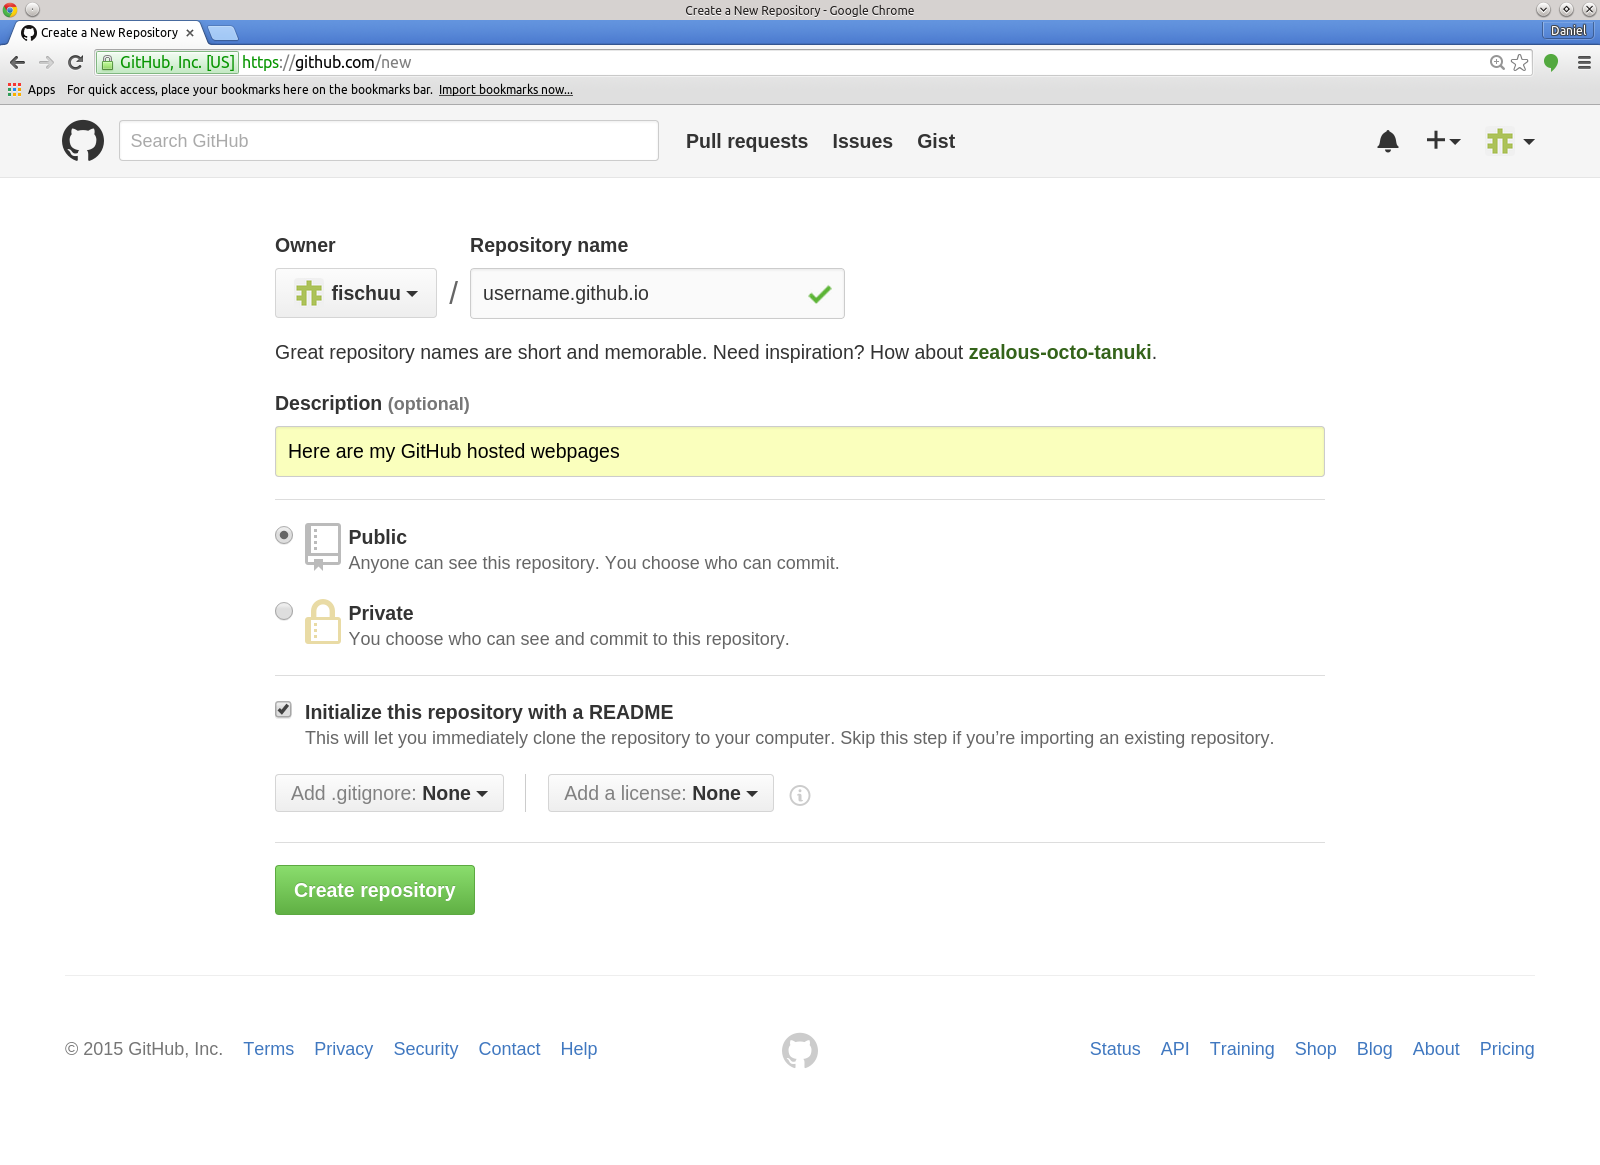
\includegraphics{assets/img/GitHub1.png}
\caption{}
\end{figure}

\begin{center}\rule{0.5\linewidth}{\linethickness}\end{center}

\subsection{Cloning to RStudio I}\label{cloning-to-rstudio-i}

\begin{itemize}
\tightlist
\item
  It is important to tick the box
\end{itemize}

\emph{Initialize this repository with a README}

\begin{itemize}
\item
  Having an initial README file in the repository enables us to clone it
  without any further problems.
\item
  From the repository we get then its address (either HTTPS, SSH or
  Subversion)
\item
  For RStudio we should copy the SSH address, e.g.~in my case:
\end{itemize}

git@github.com:fischuu/fischuu.github.io.git

\begin{itemize}
\tightlist
\item
  We start RStudio and create a new project.
\end{itemize}

\begin{center}\rule{0.5\linewidth}{\linethickness}\end{center}

\subsection{Cloning to RStudio II}\label{cloning-to-rstudio-ii}

\begin{figure}[htbp]
\centering
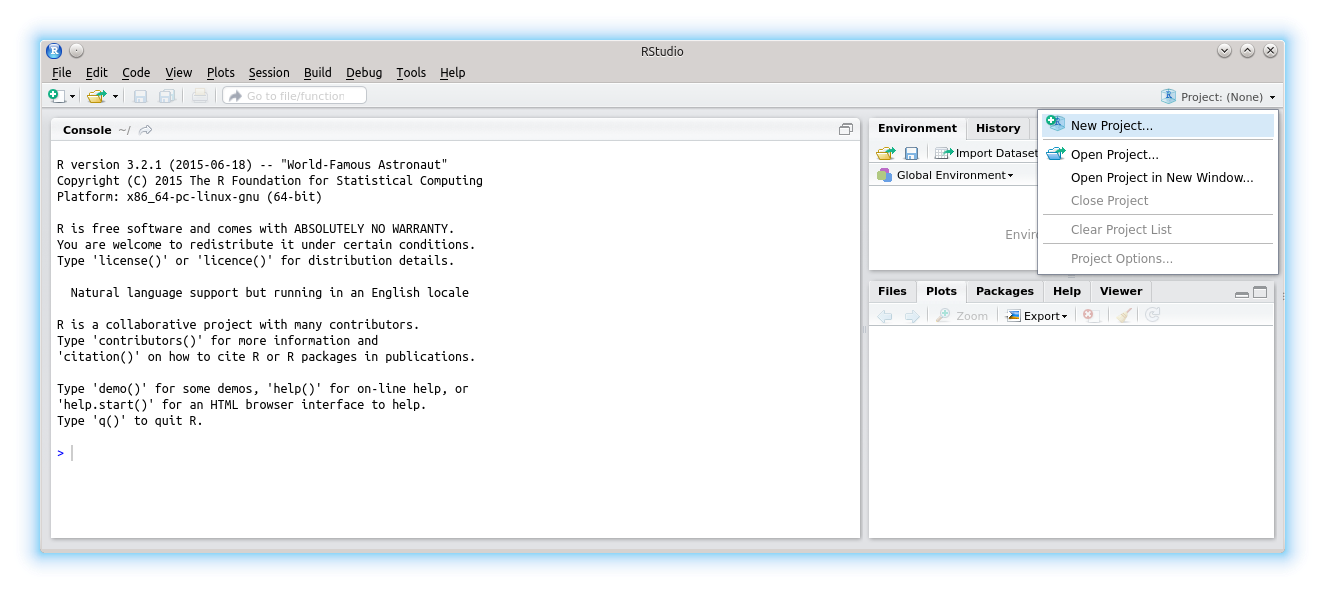
\includegraphics{assets/img/RStudio1.png}
\caption{}
\end{figure}

\begin{center}\rule{0.5\linewidth}{\linethickness}\end{center}

\subsection{Cloning to RStudio III}\label{cloning-to-rstudio-iii}

\begin{figure}[htbp]
\centering
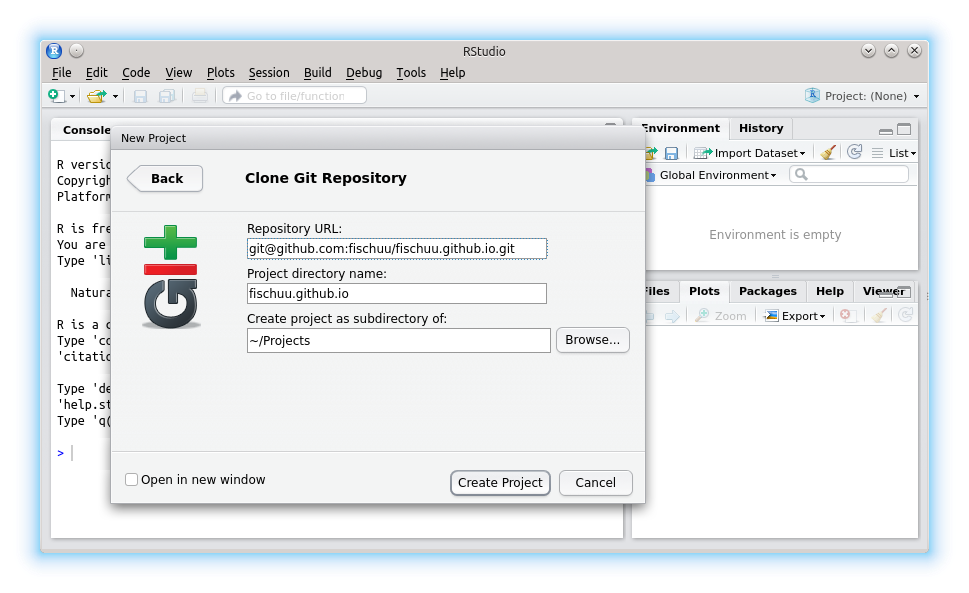
\includegraphics{assets/img/RStudio2.png}
\caption{}
\end{figure}

\begin{center}\rule{0.5\linewidth}{\linethickness}\end{center}

\subsection{Cloning to RStudio IV}\label{cloning-to-rstudio-iv}

\begin{itemize}
\tightlist
\item
  In the dialog we choose
\end{itemize}

\begin{enumerate}
\def\labelenumi{\arabic{enumi}.}
\item
  Version Control
\item
  Git
\item
  And then we provide the URL (as SSH) of the repository, the name and
  location on HDD
\end{enumerate}

\begin{itemize}
\item
  Then, we click on \emph{`Create Project'}
\item
  RStudio clones into the repository creates the folder/file structure
  on the HDD
\item
  Now we can create an own folder structure (e.g. \emph{presentations},
  \emph{lectures}, etc.)
\item
  After those steps, we have succesful connected RStudio with GitHub
  pages and we can control the repository entirely with RStudio.
\end{itemize}

\begin{center}\rule{0.5\linewidth}{\linethickness}\end{center}

\subsection{Cloning to RStudio V}\label{cloning-to-rstudio-v}

\begin{figure}[htbp]
\centering
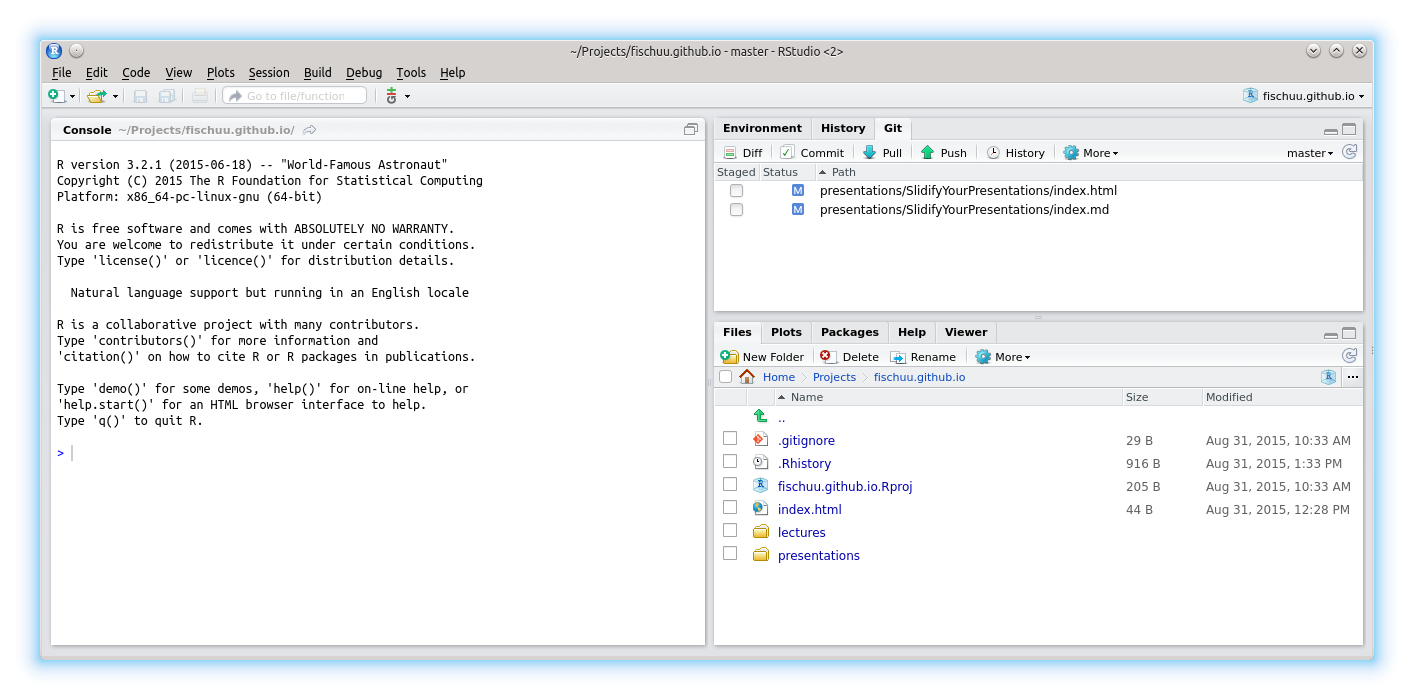
\includegraphics{assets/img/RStudio3.png}
\caption{}
\end{figure}

\begin{center}\rule{0.5\linewidth}{\linethickness}\end{center}

\subsection{Starting a new
presentation}\label{starting-a-new-presentation}

\begin{itemize}
\tightlist
\item
  To create a new presentation, we run
\end{itemize}

\begin{Shaded}
\begin{Highlighting}[]
\KeywordTok{library}\NormalTok{(}\StringTok{"slidify"}\NormalTok{)}
\KeywordTok{setwd}\NormalTok{(}\StringTok{"/home/ejo138/Projects/fischuu.github.io/presentations/"}\NormalTok{)}
\KeywordTok{author}\NormalTok{(}\StringTok{"MyFirstPresentation"}\NormalTok{, }\DataTypeTok{use_git =} \OtherTok{FALSE}\NormalTok{)}
\end{Highlighting}
\end{Shaded}

\begin{itemize}
\item
  The part \texttt{use\_git\ =\ FALSE} might be irritating, but it is
  needed, as \emph{slidify} would create otherwise a new git structure
  within the existing one (what is possible but would lead to far for
  now.)
\item
  Slidify then creates all required files and you are ready to go.
\item
  To create slides with Slidify no HTML knowledge is required, as
  everything is done via R
  \href{https://en.wikipedia.org/wiki/Markdown}{Markdown}.
\item
  Markdown is a lightweight markup language with plain text formatting
  that can be transformed into HTML (or other languages).
\end{itemize}

\begin{center}\rule{0.5\linewidth}{\linethickness}\end{center}

\subsection{\texorpdfstring{Output of
\texttt{author()}}{Output of author()}}\label{output-of-author}

\begin{itemize}
\item
  The function \texttt{author()} creates several files and folders in
  the working directory.
\item
  The main folder is called as defined in the \texttt{author()} call.
\item
  Within that folder, two more folders called \texttt{assets} and
  \texttt{libraries} are created.
\item
  The main document is called \texttt{index.Rmd}
\item
  \texttt{index.Rmd} contains two main code chunks. The header written
  in YAML defines the meta-information of the document.
\item
  The body contains the slides and uses the R Markdown language.
\end{itemize}

\begin{center}\rule{0.5\linewidth}{\linethickness}\end{center}

\subsection{This is where we start (YAML header of
index.Rmd)}\label{this-is-where-we-start-yaml-header-of-index.rmd}

\begin{Shaded}
\begin{Highlighting}[]
\NormalTok{---}
\NormalTok{title:}\StringTok{ "null"}
\NormalTok{author:}\StringTok{ "null"}
\NormalTok{highlighter:}\StringTok{ }\NormalTok{highlight.js}
\NormalTok{output:}\StringTok{ }\NormalTok{pdf_document}
\NormalTok{job:}\StringTok{ }\NormalTok{null}
\NormalTok{knit:}\StringTok{ }\NormalTok{slidify::knit2slides}
\NormalTok{mode:}\StringTok{ }\NormalTok{selfcontained}
\NormalTok{hitheme:}\StringTok{ }\NormalTok{tomorrow}
\NormalTok{subtitle:}\StringTok{ }\NormalTok{null}
\NormalTok{framework:}\StringTok{ }\NormalTok{io2012}
\NormalTok{widgets:}\StringTok{ }\NormalTok{[]}
\NormalTok{---}

\NormalTok{## Read-And-Delete}

\DecValTok{1}\NormalTok{. Edit YAML front matter}
\NormalTok{...}
\end{Highlighting}
\end{Shaded}

\begin{center}\rule{0.5\linewidth}{\linethickness}\end{center}

\subsection{This is where we start (body of
index.Rmd)}\label{this-is-where-we-start-body-of-index.rmd}

\begin{Shaded}
\begin{Highlighting}[]
\NormalTok{...}
\NormalTok{hitheme:}\StringTok{ }\NormalTok{tomorrow}
\NormalTok{subtitle:}\StringTok{ }\NormalTok{null}
\NormalTok{framework:}\StringTok{ }\NormalTok{io2012}
\NormalTok{widgets:}\StringTok{ }\NormalTok{[]}
\NormalTok{---}

\NormalTok{## Read-And-Delete}

\DecValTok{1}\NormalTok{. Edit YAML front matter}
\DecValTok{2}\NormalTok{. Write using R Markdown}
\DecValTok{3}\NormalTok{. Use an empty line followed by three dashes to separate slides!}
\NormalTok{---}\StringTok{ }\NormalTok{.class }\CommentTok{#id }

\NormalTok{## Slide 2}
\end{Highlighting}
\end{Shaded}

\begin{center}\rule{0.5\linewidth}{\linethickness}\end{center}

\subsection{Markdown basics}\label{markdown-basics}

\begin{itemize}
\item
  R markdown is a very simple markup language that makes creating slides
  extremely fast and easy.
\item
  A reference overview can be found
  \href{http://rmarkdown.rstudio.com/authoring_basics.html}{here}
\item
  For example the
  \href{https://github.com/fischuu/fischuu.github.io/raw/master/presentations/SlidifyYourPresentations/index.Rmd}{\texttt{index.Rmd}}
  of this presentation.
\item
\end{itemize}
